\section{Economic MPC}

Motivation: (setpoint stabilization is often not primary control objective 
$\Rightarrow$ "general" cost function $L$.

Assumption: $L:\mathbb{R}^n\rightarrow\mathbb{R}^n$ is continuous (need not
be positive defined) $X,U$ is compact.

\begin{Definition}
 Optimal steady-state $(x_s,u_s)=\arg\min_{x=f(x,u);\ x\in X;\ u\in U}L(x,u)$
\end{Definition}

\begin{Example}
 \begin{equation*}
  \begin{split}
   &x^+=xu \\
   &X=U=[-\delta,\delta] \\
   &L(x,u)=g(x)+(u+1)^2
  \end{split}
 \end{equation*}
 
 \begin{center}
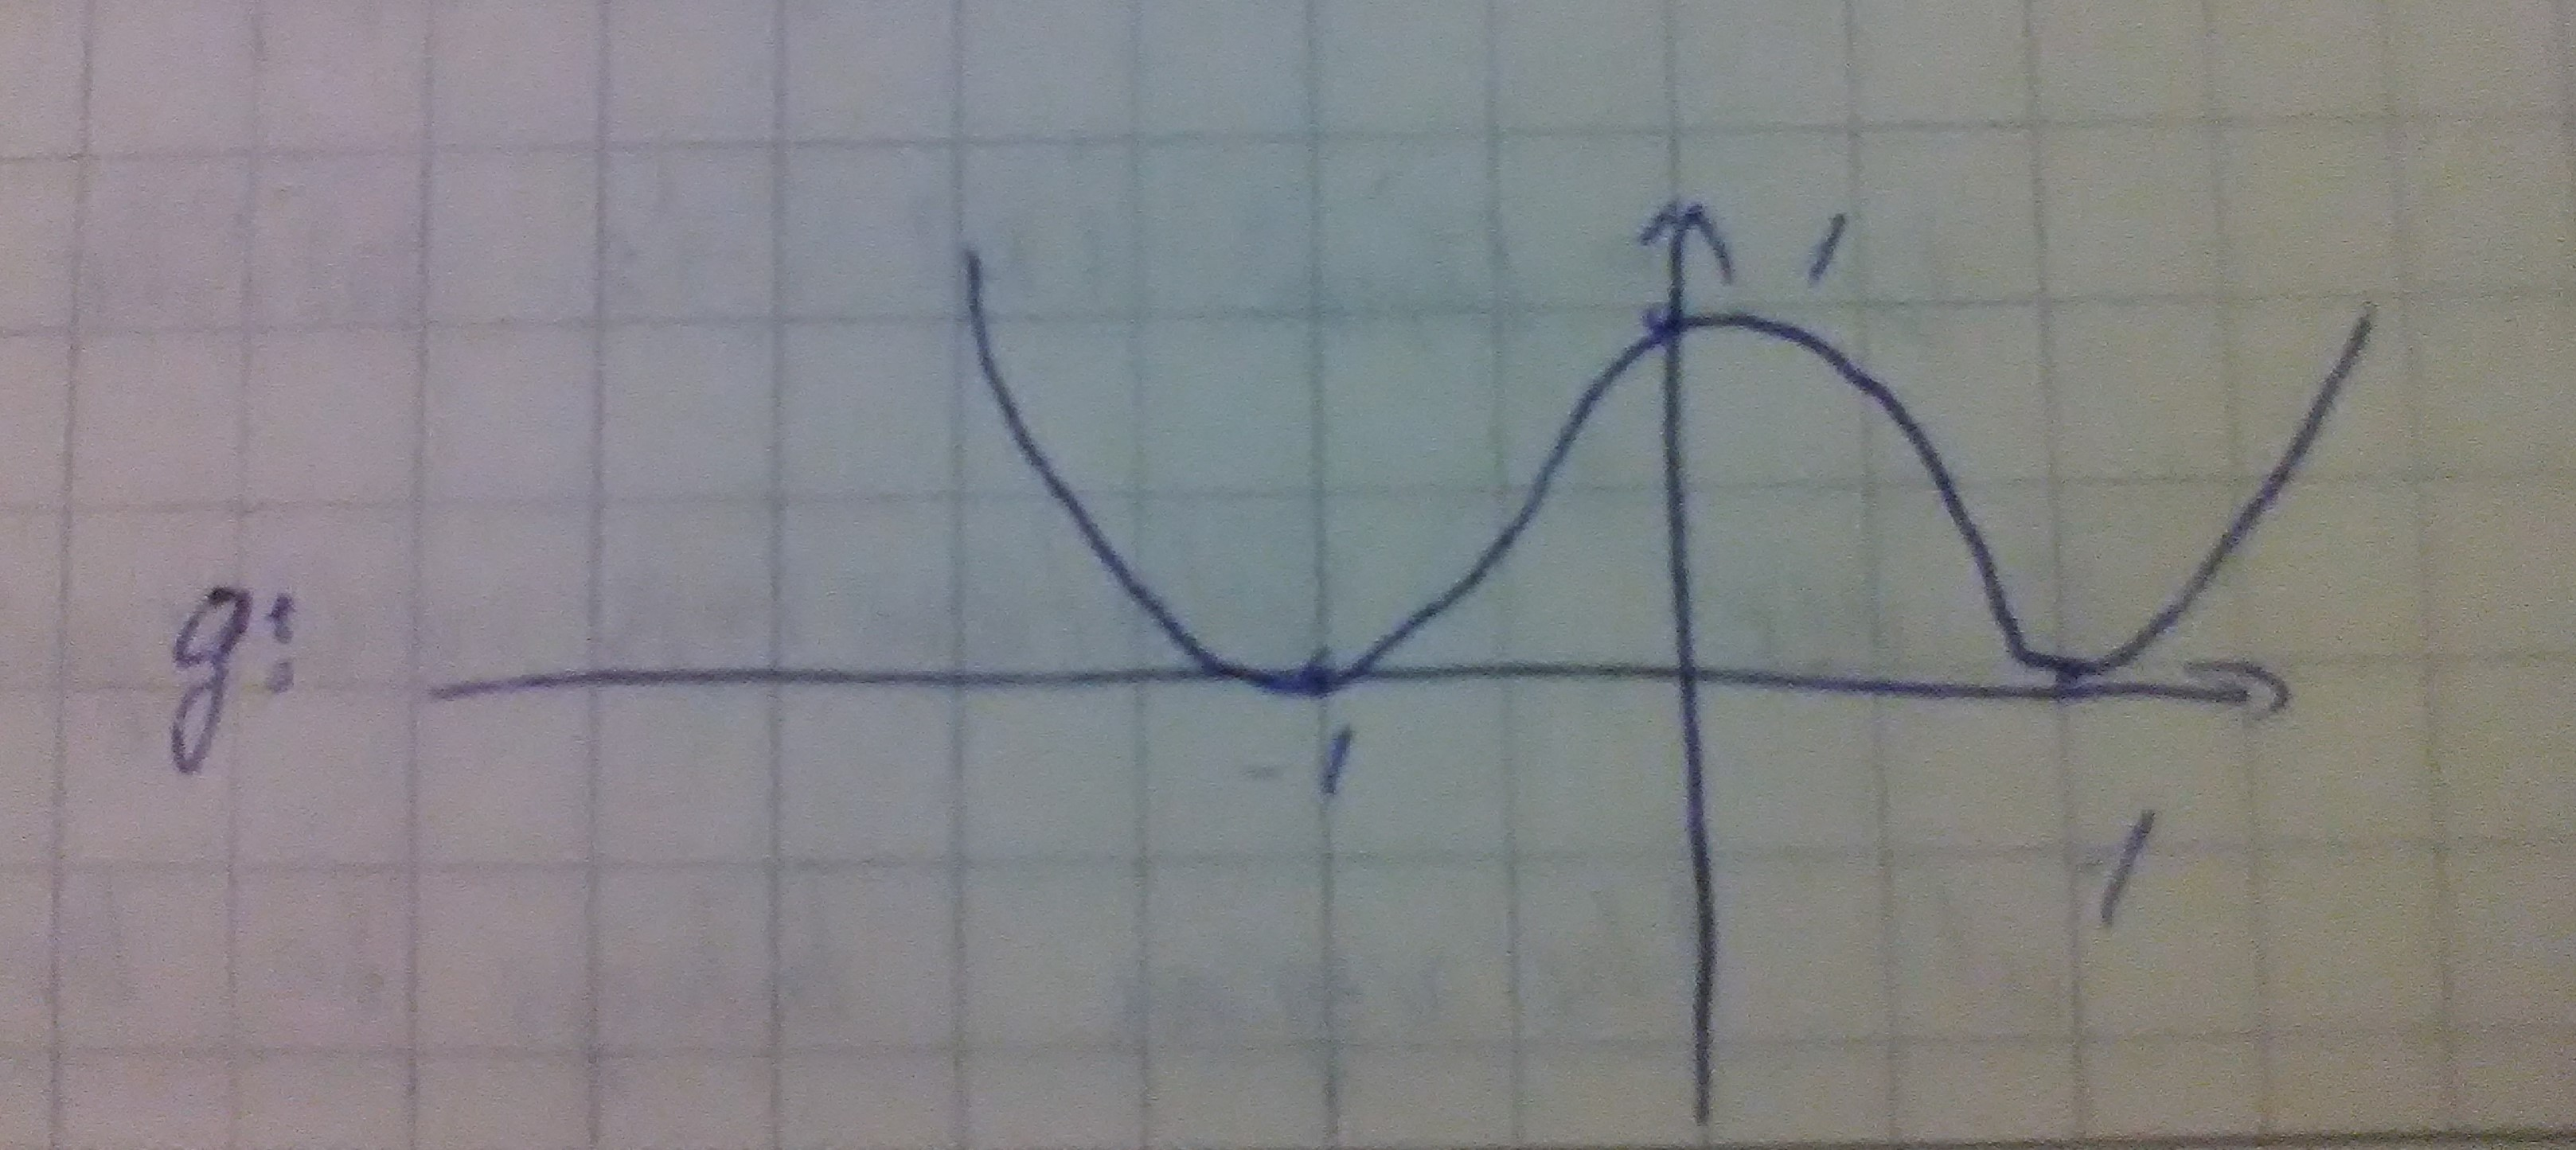
\includegraphics[scale=0.1]{3}
\end{center}

 Optimal steady state is $(x_s,u_s)=(0,-1)$

 Optimal operating condition:

 \begin{equation*}
  \begin{split}
   &x=(-1;+1;-1;\dots) \\
   &u=(-1;-1;-1;\dots)
  \end{split}
 \end{equation*}
\end{Example}


Economic MPC problem

At each time $t$, given $x(t)$, we should minimize $J(x(t),u(\cdot|t))$ s.t.

$$J(x(t),u(\cdot|t) = \sum_{k=t}^{t+N-1}L(x(k|t),u(k|t))$$

With conditions:

\begin{equation*}
 \begin{split}
  &x(k+1|t) = f(x(k|t),u(k|t)) \\
  &x(t|t) = x(t) \\
  &x(k|t)\in X \\
  &u(k|t)\in U \\
  &x(t+N|t) = x_s
 \end{split}
\end{equation*}

Remark: this can be extended to terminal region/cost framework.

Closed-loop average performance

\begin{Theorem}
 The closed-loop asymptotic average performance is at least as good as the
 optimal steady-state cost i.e.,

 $$\lim_{T\rightarrow\infty}\sup\frac{\sum_{k=0}^{T-1}L(x(k),u(k)}{T}\le L(x_s,u_s)$$

 \begin{proof}
  Lets present a completely new way of proving that we have not used before 
  in this course.

  Joke. We again consider difference $J^*(x(t+1))-J^*(x(t))$.

  $$J^*(x(t+1))-J^*(x(t))\le -L(x(t),u(t)) + L(x_s,u_s)$$

  From this equation we can get:

  $$\frac{\sum_{k=0}^{T-1}\left(J^*(x(k+1))-J^*(x(k))\right)}{T}\le\frac{\sum_{k=0}^{T-1}\left(L(x_s,u_s)+-L(x(t),u(t))\right)}{T}$$

  \begin{equation}\label{eq:EMPC1}
   \begin{split}
    \lim_{T\rightarrow\infty}\inf LHS \le &\lim_{T\rightarrow\infty}\inf RHS = \\
    &= L(x_s,u_s)+\lim_{T\rightarrow\infty}\inf\frac{\sum_{k=0}^{T-1}-L(x(k),u(k))}{T} = \\
    &= L(x_s,u_s)-\lim_{T\rightarrow\infty}\sup\frac{\sum_{k=0}^{T-1}L(x(k),u(k))}{T} 
   \end{split}
  \end{equation}

  Also, we can rewrite

  \begin{equation}\label{eq:EMPC2}
   \begin{split}
    \frac{\sum_{k=0}^{T-1}\left(J^*(x(k+1))-J^*(x(k))\right)}{T}=&\lim_{T\rightarrow\infty}\inf\frac{J^*(x(T))-J^*(x(0))}{T} \ge \\
                       &\ge\lim_{T\rightarrow\infty}\inf\frac{-J^*(x(0))}{T} = 0
   \end{split}
  \end{equation}

  Now combine (\ref{eq:EMPC1}) and (\ref{eq:EMPC2}) and we get

  $$\lim_{T\rightarrow\infty}\sup\frac{\sum_{k=0}^{T-1}L(x(k),u(k))}{T} \le L(x_s,u_s)$$
 \end{proof}
\end{Theorem}


Classify optimal operating condition

\begin{Definition}
 A system is optimally operated at steady-state if
 $$\lim_{T\rightarrow\infty}\inf\frac{\sum_{k=0}^{T-1}L(x(k),u(k))}{T} \ge L(x_s,u_s)$$

 for all feasible sequences $(x(\cdot), u(\cdot))$.
\end{Definition}

\begin{Definition}
 A system is dissipative w.r.t. supply rate $s(x,u)$ if there exists a storage 
 function $\lambda:X\rightarrow\mathbb{R}_{\ge 0}$ s.t.
 $$\lambda(f(x,u))-\lambda(x)\le s(x,u)$$

 For strictly dissipativity RHS=$s(x,u)-\rho((x-x_0))$, where $\rho$ positive defined.
\end{Definition}

\begin{Theorem}
 A system is optimally operated at steady state if it is dissipative w.r.t.
 $s(x,u)=L(x,u)-L(x_s,u_s)$.
 \begin{proof}
  \begin{equation}
   \begin{split}
    \lim_{T\rightarrow\infty}\inf\frac{\sum_{t=0}^{T-1}\lambda(x(t+1))-\lambda(x(t))}{T} &\le
           \lim_{T\rightarrow\infty}\inf\frac{\sum_{t=0}^{T-1}s(x(t),u(t))}{T}= \\
           &=\lim_{T\rightarrow\infty}\inf\frac{\sum_{t=0}^{T-1}L(x(t),u(t))}{T}-L(x_s,u_s)
   \end{split}
  \end{equation}

  Note, that $\lim_{T\rightarrow\infty}\inf\frac{\sum_{t=0}^{T-1}\lambda(x(t+1))-\lambda(x(t))}{T} \ge 0$
 \end{proof}
\end{Theorem}


\begin{Example}
 Consider system
 \begin{equation}
  \begin{split}
   &x(t+1)=x(t)u(t) \\
   &X=U=[-5,5] \\
   &L(x,u)=(x-1)^2+\delta(u-2)^2,\ \ 0<\delta<1
  \end{split}
 \end{equation}

 Set of all feasible steady-states $\{(x,u)|x=0\ \ or \ \ u=1 \}$. Let $(x_s,u_s)=(1,1)$, then
 $L(x_s,u_s)=\delta$.

 $s(x,u)=L(x,u)-L(x_s,u_s)=(x-1)^2+\delta(u-2)^2-\delta$, we will search $\lambda(x)$ in form
 $$\lambda(x)=ax+c$$

 From dissipativity enequation we shooud have $\lambda(f(x,u))-\lambda(x)\le s(x,u)$, then
 compare $\lambda(f(x,u))-\lambda(x)=axu-ax$ with $s(x,u)=(x-1)^2+\delta(u-2)^2-\delta$.

 Consider $s(x,u)-(\lambda(f(x,u))-\lambda(x))=g(x,u)$ as function, and find parameters $a$ such
 that $g(x,u)\ge0$, $\forall x\in X,\ \ u\in U$. And minimum in point $(x_s,u_s)=(1,1)$
 $$\triangledown g(x,u)=\left[
  \begin{tabular}{l}
   $2(x-1)-au+a$ \\ 
   $2\delta(u-2) -a x$ 
  \end{tabular} 
 \right]$$

 Function $g$ is convex.

 $$\left[
  \begin{tabular}{l}
   $2(x-1)-au+a$ \\ 
   $2\delta(u-2) -a x$ 
  \end{tabular} 
 \right]_{(1,1)} = 0$$ 

 Thus $a = -2\delta$, and from requrements, that $\lambda(x)=ax+c\ge 0\ \ \forall x\in X=[-5,5]$
 we have $c\ge -ax = 2\delta x \ge [x=5] \ge 10\delta$.\

 And now we can use previous theorem to prove, that system is optimaly operated at
 steady state $(x_s,u_s)=(1,1)$.

 Consider case, when system is not dissipative. Change previous constraint for $u$, let $u\le 0$:
 then new optimal steady-state $(x_s,u_s)=(0,0)$ and $L(x_s,u_s)=4\delta+1$.

 Consider 2-period orbits:

 \begin{equation}
  \begin{split}
   &x(\cdot) = (1,-\frac{1}{3},1,-\frac{1}{3},\dots)\\
   &u(\cdot) = (-\frac{1}{3},-3,-\frac{1}{3},-3,\dots)
  \end{split}
 \end{equation}

 With this orbits

 $$\lim_{T\rightarrow\infty}\inf\frac{\sum_{t=0}^{T-1}L(x(t),u(t))}{T}=\frac{L(1,-\frac{1}{3})+L(-\frac{1}{3},-3)}{2}=
 \frac{(\frac{4}{3})^2}{2}+\delta\frac{\frac{-7}{3}+(-3)^2}{2}$$

  And for small enough $\delta$ this less then $L(0,0)$. That mean, that system is not optimal 
  operated at steady state and not dissipative w.r.t. chosen $s(x,u)$. 


\end{Example}

Closed-loop convergence to the optimal steady state

\begin{Theorem}
Suppose the system is strictly dissipative w.r.t. the supply rate $s(x,u) = L(x,u) - L(x_s, u_s)$. Then the closed-loop system asymptotically converge to the optimal steady state $x_s$.

Remark: $x_s$ is asymptotically stable if $J^*(x)$ and $\lambda(x)$ are continuous at $x_s$.
\begin{proof}
Define "rotated" cost function
\begin{equation*}
\tilde{L}(x,u) =L(x,u) - L(x_s, u_s) + \lambda(x) - \lambda(f(x,u))
\end{equation*}

Auxiliary optimization problem $\tilde{P}$
\begin{equation*}
\min_{u(\cdot| t)} \tilde{J}(x(t),u(t)) = \sum_{k=t}^{t+N-1}\tilde{L}(x(k|t),u(k|t))
\end{equation*}

s.t. some constraints as in original MPC problem

Claim: $P$ and $\tilde{P}$ have the same minimizer. 
Proof of claim: feasible sets coincide 
\begin{equation*}
\begin{split}
\tilde{J}(x(t),u(t)) &= \sum_{k=t}^{t+N-1} [L(x(k|t),u(k|t)) + \lambda(x(k|t)) - \lambda(f(x(k|t),u(k|t))) - L(x_s,u_s)]= \\
&= \lambda(x(t|t)) - \lambda(x(t+N|t)) - NL(x_s,u_s) + \sum_{k=1}^{t+N-1}L(x(k|t),u(k|t))= \\
&= \lambda(x(t)) - \lambda(x_s) - NL(x_s,u_s) + J(x(t),u(\cdot | t))
\end{split}
\end{equation*}
$\Rightarrow \tilde{J}$ and $J$ only differ by a constant $\Rightarrow P$ and $\tilde{P}$ have the same minimizer.

$\Rightarrow$ we can use $\tilde{P}$ to analyze stability of the closed loop. $\tilde{L}(x,u) \geq \rho (|x - x_s|)$, $\tilde{L}$ is positive definite (from strictly dissipative) $\Rightarrow$ can apply standard MPC stability results.  
\end{proof}
\end{Theorem}

Average constraints:

\begin{Definition}
Asymptotic average constraints $h: \mathbb{R}^n \times \mathbb{R}^m \to \mathbb{R}^p$ - (auxiliary) output specifying average constraints.
\end{Definition}

Assumption: $h$ is continuous
\begin{itemize}
\item $Av[h(x,u)] \in Y$
\item $Av[h(x,u)] := \{ \bar{h}: \exists {t_n} \to \infty \ s.t. \ \lim_{n \to \infty} \frac{\sum_{t=0}^{t_n - 1}h(x(t),u(t))}{t_n}  = \bar{h}\}$

$Av[h(x,u)]$ "set of asymptotic average values of $h$".
\end{itemize}

How to modify the MPC problem accordingly?

Adaptation of optimal steady state computation
\begin{equation*}
(x_s,u_s) = arg\,min_{x = f(x,u), x \in X, u \in U, h(x,u) \in Y} L(x,u)
\end{equation*}

Additional constraint:
\begin{equation*}
\sum_{k=t}^{t+N-1}h(x(k|t),u(k|t)) \in Y_t
\end{equation*}
with $Y_{t+1} := Y_t \oplus Y \oplus {-h(x(t),u(t))}$, $Y_0 = NY \oplus Y_{00}$, $Y_{00}$ - arbitrary compact set.

\begin{enumerate}
\item How to guarantee recursive feasibility?

Candidate solution at time $t+1$ 
\begin{equation*}
\tilde{u}(k|t+1) = \left \{
  \begin{tabular}{ll}
  $u^*(k|t)$ & $\ t+1 \leq k \leq t+N+1$ \\
  $u_s$ & $\ k = t + N$
  \end{tabular}
\right .
\end{equation*}
\begin{equation*}
\sum_{k=t+1}^{t+N}h(\tilde{x}(k|t+1), \tilde{u}(k|t+1)) = \sum_{k=t}^{t+N-1}h(x^*(k|t), u^*(k|t))[\in Y_t] - h(x(t),u(t)) + h(x_s,u_s)[\in Y]
\end{equation*}
$\in Y_t \oplus Y \oplus {-h(x(t),u(t))} = Y_{t+1}$
\item Satisfaction of average constraint for the resulting closed loop:

Assumption: $Y$ is convex. Solve the recursion for $Y_t$ to obtain 
\begin{equation*}
Y_t = Y_{00} \oplus (t+N)Y \oplus {- \sum_{k=0}^{t-1}h(x(k),u(k))}
\end{equation*}
the last item is closed loop sequence.

From the additional constraint in optimal problem:
\begin{equation*}
\sum_{k=0}^{t-1}h(x(k),u(k)) + \sum_{k=t}^{t+N-1}h(x(k|t), u(k|t)) \in Y_{00} \oplus (t+N)Y
\end{equation*}

For each sequence {$t_n$} s.t. $\lim_{n \to \infty} \sum_{k=0}^{t_n -1}\frac{h(x(k),u(k))}{t_n} $ exists, we obtain 
\begin{equation*}
\lim_{n \to \infty} \frac{\sum_{k=0}^{t_n-1}h(x(k),u(k))}{t_n} \in \lim_{n \to \infty} \frac{Y_{00} \oplus (t_n + N)Y}{t_n} = Y
\end{equation*}
$\Rightarrow$ closed-loop system satisfies average constraints.
\end{enumerate}

Now lets consider additional constraint (Transient average constraint):
\begin{equation*}
\sum_{k=t}^{t+T-1}\frac{h(x(k),u(k))}{T} \in Y, \ \forall t \geq 0
\end{equation*}
for $T=1$, standard pointwise-in-time 

This constraint add some additional constraints for $h(x,u)$. Lets assume, that: $Y= \mathbb{R}^p_{\leq 0}$, now we can 
$T+N-1$ constraints in total,described below:

\begin{equation*}
\left \{
\begin{tabular}{l} 
$\sum_{t-T+\tau}^{t-1} h(x(k),u(k)) + \sum_{i=t}^{t+\tau -1}h(x(i|t), u(i|t)) \le 0 \ \tau = 1, ..., T$ \\
$\sum_{i=t+j+1}^{t+T+j}h(x(i|t),u(i|t)) \leq 0, \ j =0, ..., N-2$ \\
$u(i|t) = u_s \ i = t+N, ... , t+N-2+T$ 
\end{tabular} 
\right .  
\end{equation*}

\begin{itemize}
\item recursive feasibility can be shown using standard candidate sequence
\item closed-loop transient average constraint satisfaction directly follows from first additional constraint
\end{itemize}